% interactcadsample.tex
% v1.03 - April 2017

\documentclass[]{interact}

\usepackage{epstopdf}% To incorporate .eps illustrations using PDFLaTeX, etc.
\usepackage{subfigure}% Support for small, `sub' figures and tables
%\usepackage[nolists,tablesfirst]{endfloat}% To `separate' figures and tables from text if required

\usepackage{natbib}% Citation support using natbib.sty
\bibpunct[, ]{(}{)}{;}{a}{}{,}% Citation support using natbib.sty
\renewcommand\bibfont{\fontsize{10}{12}\selectfont}% Bibliography support using natbib.sty

\theoremstyle{plain}% Theorem-like structures provided by amsthm.sty
\newtheorem{theorem}{Theorem}[section]
\newtheorem{lemma}[theorem]{Lemma}
\newtheorem{corollary}[theorem]{Corollary}
\newtheorem{proposition}[theorem]{Proposition}

\theoremstyle{definition}
\newtheorem{definition}[theorem]{Definition}
\newtheorem{example}[theorem]{Example}

\theoremstyle{remark}
\newtheorem{remark}{Remark}
\newtheorem{notation}{Notation}

% Pandoc syntax highlighting
\usepackage{color}
\usepackage{fancyvrb}
\newcommand{\VerbBar}{|}
\newcommand{\VERB}{\Verb[commandchars=\\\{\}]}
\DefineVerbatimEnvironment{Highlighting}{Verbatim}{commandchars=\\\{\}}
% Add ',fontsize=\small' for more characters per line
\usepackage{framed}
\definecolor{shadecolor}{RGB}{248,248,248}
\newenvironment{Shaded}{\begin{snugshade}}{\end{snugshade}}
\newcommand{\AlertTok}[1]{\textcolor[rgb]{0.94,0.16,0.16}{#1}}
\newcommand{\AnnotationTok}[1]{\textcolor[rgb]{0.56,0.35,0.01}{\textbf{\textit{#1}}}}
\newcommand{\AttributeTok}[1]{\textcolor[rgb]{0.77,0.63,0.00}{#1}}
\newcommand{\BaseNTok}[1]{\textcolor[rgb]{0.00,0.00,0.81}{#1}}
\newcommand{\BuiltInTok}[1]{#1}
\newcommand{\CharTok}[1]{\textcolor[rgb]{0.31,0.60,0.02}{#1}}
\newcommand{\CommentTok}[1]{\textcolor[rgb]{0.56,0.35,0.01}{\textit{#1}}}
\newcommand{\CommentVarTok}[1]{\textcolor[rgb]{0.56,0.35,0.01}{\textbf{\textit{#1}}}}
\newcommand{\ConstantTok}[1]{\textcolor[rgb]{0.00,0.00,0.00}{#1}}
\newcommand{\ControlFlowTok}[1]{\textcolor[rgb]{0.13,0.29,0.53}{\textbf{#1}}}
\newcommand{\DataTypeTok}[1]{\textcolor[rgb]{0.13,0.29,0.53}{#1}}
\newcommand{\DecValTok}[1]{\textcolor[rgb]{0.00,0.00,0.81}{#1}}
\newcommand{\DocumentationTok}[1]{\textcolor[rgb]{0.56,0.35,0.01}{\textbf{\textit{#1}}}}
\newcommand{\ErrorTok}[1]{\textcolor[rgb]{0.64,0.00,0.00}{\textbf{#1}}}
\newcommand{\ExtensionTok}[1]{#1}
\newcommand{\FloatTok}[1]{\textcolor[rgb]{0.00,0.00,0.81}{#1}}
\newcommand{\FunctionTok}[1]{\textcolor[rgb]{0.00,0.00,0.00}{#1}}
\newcommand{\ImportTok}[1]{#1}
\newcommand{\InformationTok}[1]{\textcolor[rgb]{0.56,0.35,0.01}{\textbf{\textit{#1}}}}
\newcommand{\KeywordTok}[1]{\textcolor[rgb]{0.13,0.29,0.53}{\textbf{#1}}}
\newcommand{\NormalTok}[1]{#1}
\newcommand{\OperatorTok}[1]{\textcolor[rgb]{0.81,0.36,0.00}{\textbf{#1}}}
\newcommand{\OtherTok}[1]{\textcolor[rgb]{0.56,0.35,0.01}{#1}}
\newcommand{\PreprocessorTok}[1]{\textcolor[rgb]{0.56,0.35,0.01}{\textit{#1}}}
\newcommand{\RegionMarkerTok}[1]{#1}
\newcommand{\SpecialCharTok}[1]{\textcolor[rgb]{0.00,0.00,0.00}{#1}}
\newcommand{\SpecialStringTok}[1]{\textcolor[rgb]{0.31,0.60,0.02}{#1}}
\newcommand{\StringTok}[1]{\textcolor[rgb]{0.31,0.60,0.02}{#1}}
\newcommand{\VariableTok}[1]{\textcolor[rgb]{0.00,0.00,0.00}{#1}}
\newcommand{\VerbatimStringTok}[1]{\textcolor[rgb]{0.31,0.60,0.02}{#1}}
\newcommand{\WarningTok}[1]{\textcolor[rgb]{0.56,0.35,0.01}{\textbf{\textit{#1}}}}

% tightlist command for lists without linebreak
\providecommand{\tightlist}{%
  \setlength{\itemsep}{0pt}\setlength{\parskip}{0pt}}

% From pandoc table feature
\usepackage{longtable,booktabs,array}
\usepackage{calc} % for calculating minipage widths
% Correct order of tables after \paragraph or \subparagraph
\usepackage{etoolbox}
\makeatletter
\patchcmd\longtable{\par}{\if@noskipsec\mbox{}\fi\par}{}{}
\makeatother
% Allow footnotes in longtable head/foot
\IfFileExists{footnotehyper.sty}{\usepackage{footnotehyper}}{\usepackage{footnote}}
\makesavenoteenv{longtable}


\usepackage{hyperref}
\usepackage[utf8]{inputenc}
\def\tightlist{}
\hypersetup{
  colorlinks=true,
  citecolor = cyan,
  linkcolor=blue,
  filecolor=magenta,      
  urlcolor=blue
  }

\usepackage{float}

\begin{document}


\articletype{PREPRINT}

\title{Exploring Equivalence Testing with the Updated TOSTER R Package}


\author{\name{Aaron R. Caldwell$^{a}$}
\affil{$^{a}$Natick, MA, \url{https://orcid.org/0000-0002-4541-6283}}
}

\thanks{CONTACT Aaron R.
Caldwell. Email: \href{mailto:arcaldwell49@gmail.com}{\nolinkurl{arcaldwell49@gmail.com}}}

\maketitle

\begin{abstract}
This is an article detailing the ``avocado TOST'' update to the TOSTER R
package.
\end{abstract}

\begin{keywords}
statistics, bootstrapping, minimal effects test, NHST, TOST
\end{keywords}

\hypertarget{introduction}{%
\section{Introduction}\label{introduction}}

Researchers often erroneously declare that no statistical effect exists
based on a single ``non-significant'' p-value \citep{blandaltman95}. In
many of these cases, the data may corroborate the researchers claim but
the interpretation of a null hypothesis significance test (NHST),
wherein the null hypothesis is ``no effect'', is nonetheless incorrect.
In order to statistically test for whether there is ``no effect'' or
``no difference'' researchers could explore using equivalence testing. A
very simple equivalence testing approach is the use of ``two one-sided
tests'' (TOST) \citep{schuirmann1987}. In TOST procedures, an upper
(\(\Delta_U\)) and lower (\(\Delta_L\)) equivalence bound is specified
based on the smallest effect size of interest (SESOI). If the TOST is
below a pre-specified alpha level, then the effect can be considered
close enough to zero to be practically equivalent \citep{lakens_ori}.

Both the complaints about erroneous conclusions regarding equivalence
\citep{blandaltman95} and proposed statistical solutions
\citep{schuirmann1987} have existed for decades now. Yet the problem
appears to persist in many applied disciplines. I estimate that the
cause of this continued dissonance is due to a lack of education on
equivalence testing and a struggle for many applied researchers to
implement equivalence testing. In my experience, most researchers have
received some degree of statistical training in their doctoral or
master's studies, but it is rare that any have idea of how to use TOST.
It may also be difficult to implement equivalence testing for many
researchers. This may be caused by most statistical software defaulting
to a null hypothesis of zero, or even completely lacking an ability to
change the null hypothesis. Therefore, I feel continued development of
educational content on TOST, and software to help with such analyses,
would be beneficial to many quantitative researchers.

The TOSTER R package was originally developed in by \citet{lakens_ori}
to introduce experimental psychologists to the concept of equivalence
testing and provide an easy-to-use implementation in R. In the years
since that publication, I have made a significant update to the package
in order to improve the user interface and expand the tools available
within the package. An experienced R programmer may have no problem
performing equivalence testing within R but beginners may struggle with
both writing the code and interpreting the output. If you fall into that
category, I would suggest using \texttt{jamovi}, an open-source
statistical software, that has a TOSTER module to perform
equivalence/TOST analyses.

In this manuscript, I will detail the updates to the TOSTER package, and
give some basic usage examples of some of the new functions. This is
meant to just be an introduction to \emph{how} to perform such analyses,
and provide a little bit of context for when such analyses are
appropriate. For a greater introduction to equivalence testing, I would
suggest reading other methodological tutorials
\citep{lakens_ori, lakens2018equivalence, lakens2020improving, mazzolari2022myths}.

\hypertarget{basics-of-equivalence-testing}{%
\section{Basics of Equivalence
Testing}\label{basics-of-equivalence-testing}}

\hypertarget{the-toster-r-package}{%
\subsection{The TOSTER R Package}\label{the-toster-r-package}}

In an effort to make TOSTER more informative and easier to use, a new
function \texttt{t\_TOST} was created. This function operates very
similarly to base R's \texttt{t.test} function, but performs 3 t-tests
(one two-tailed and two one-tailed tests). In addition, this function
has a generic method where two vectors can be supplied or a formula can
be given (e.g.,\texttt{y\ \textasciitilde{}\ group}). This function also
makes it easier to switch between types of t-tests. All three types (two
sample, one sample, and paired samples) can be performed/calculated from
the same function. Moreover, the output from this function is verbose,
and should make the decisions derived from the function more informative
and user-friendly.

Also, \texttt{t\_TOST} is not limited to equivalence tests. Minimal
effects testing (MET) is possible. MET is useful for situations where
the hypothesis is about a minimal effect and the null hypothesis
\emph{is} equivalence (see Figure 1).

\begin{figure}
\centering
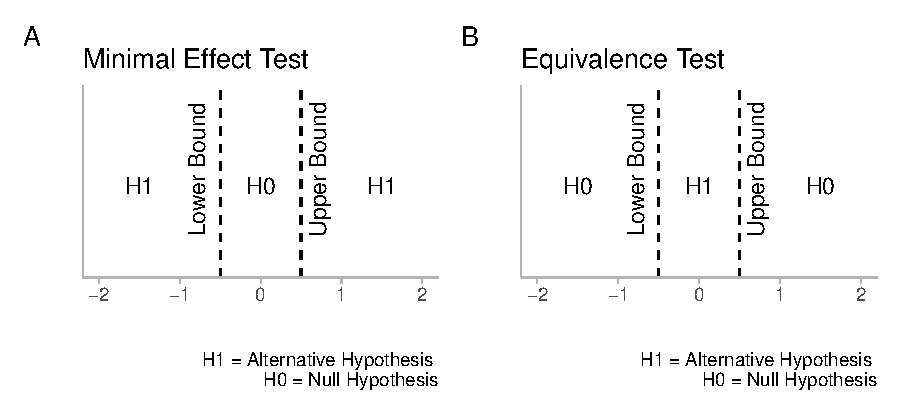
\includegraphics{Avocado_Update_files/figure-latex/hypplot-1.pdf}
\caption{Type of Hypothesis}
\end{figure}

\newpage

\hypertarget{vignettes-with-toster}{%
\subsection{Vignettes with TOSTER}\label{vignettes-with-toster}}

In the general introduction to this package we detailed how to look at
\emph{old} results and how to apply TOST to interpreting those results.
However, in many cases, users may have new data that needs to be
analyzed. Therefore, \texttt{t\_TOST} can be applied to new data. This
vignette will use the \texttt{bugs} data from the \texttt{jmv} R package
and the \texttt{sleep} data.

\begin{Shaded}
\begin{Highlighting}[]
\FunctionTok{data}\NormalTok{(}\StringTok{\textquotesingle{}sleep\textquotesingle{}}\NormalTok{)}
\FunctionTok{library}\NormalTok{(jmv)}
\FunctionTok{data}\NormalTok{(}\StringTok{\textquotesingle{}bugs\textquotesingle{}}\NormalTok{)}
\end{Highlighting}
\end{Shaded}

\hypertarget{independent-groups}{%
\subsubsection{Independent Groups}\label{independent-groups}}

For this example, we will use the sleep data. In this data there is a
\texttt{group} variable and an outcome \texttt{extra}.

\begin{Shaded}
\begin{Highlighting}[]
\FunctionTok{head}\NormalTok{(sleep,}\DecValTok{2}\NormalTok{)}
\end{Highlighting}
\end{Shaded}

\begin{verbatim}
##   extra group ID
## 1   0.7     1  1
## 2  -1.6     1  2
\end{verbatim}

We will assume the data are independent, and that we have equivalence
bounds of +/- 0.5. All we need to do is provide the \texttt{formula},
\texttt{data}, and \texttt{eqb} arguments for the function to run
appropriately. In addition, we can set the \texttt{var.equal} argument
(to assume equal variance), and the \texttt{paired} argument (sets if
the data is paired or not). Both are logical indicators that can be set
to TRUE or FALSE. The \texttt{alpha} is automatically set to 0.05 but
this can also be adjusted by the user.

Standardize mean differences (SMDs) are provided in the output for any
t-test based TOST analysis (e.g., Cohen's d). The Hedges's corrected SMD
\citep{hedges_bias} is automatically calculated, but this can be
overridden with the \texttt{bias\_correction} argument\footnote{Glass's
  delta can also be produced in the output by using the \texttt{glass}
  argument}. In previous versions of this package, the equivalence
bounds could be set by the SMD (e.g., equivalence bound of 0.5 SD), but
this is an erroneous approach since the bound would be dependent upon
the \emph{sample} variance. However, users can opt for such an analysis
by setting \texttt{eqbound\_type} to SMD, which will produce a
noticeable warning to the R console.

The \texttt{hypothesis} argument is automatically set to ``EQU'' for
equivalence but if a minimal effect is of interest then ``MET'' can be
supplied.

\begin{Shaded}
\begin{Highlighting}[]
\CommentTok{\# Formula Interface}
\NormalTok{res1 }\OtherTok{=} \FunctionTok{t\_TOST}\NormalTok{(}\AttributeTok{formula =}\NormalTok{ extra }\SpecialCharTok{\textasciitilde{}}\NormalTok{ group, }\AttributeTok{data =}\NormalTok{ sleep, }
              \AttributeTok{eqb =}\NormalTok{ .}\DecValTok{5}\NormalTok{, }\AttributeTok{smd\_ci =} \StringTok{"t"}\NormalTok{)}
\CommentTok{\# x \& y Interface}
\NormalTok{res1a }\OtherTok{=} \FunctionTok{t\_TOST}\NormalTok{(}\AttributeTok{x =} \FunctionTok{subset}\NormalTok{(sleep,group}\SpecialCharTok{==}\DecValTok{1}\NormalTok{)}\SpecialCharTok{$}\NormalTok{extra,}
               \AttributeTok{y =} \FunctionTok{subset}\NormalTok{(sleep,group}\SpecialCharTok{==}\DecValTok{2}\NormalTok{)}\SpecialCharTok{$}\NormalTok{extra, }\AttributeTok{eqb =}\NormalTok{.}\DecValTok{5}\NormalTok{)}
\end{Highlighting}
\end{Shaded}

\newpage

Once the function has run, we can print the results with the
\texttt{print} method. This provides a verbose summary of the results.

\begin{Shaded}
\begin{Highlighting}[]
\FunctionTok{print}\NormalTok{(res1)}
\end{Highlighting}
\end{Shaded}

\begin{verbatim}
## 
## Welch Two Sample t-test
## 
## The equivalence test was non-significant, t(17.78) = -1.272, p = 8.9e-01
## The null hypothesis test was non-significant, t(17.78) = -1.861, p = 7.94e-02
## NHST: don't reject null significance hypothesis that the effect is equal to zero 
## TOST: don't reject null equivalence hypothesis
## 
## TOST Results 
##                 t    df p.value
## t-test     -1.861 17.78   0.079
## TOST Lower -1.272 17.78   0.890
## TOST Upper -2.450 17.78   0.012
## 
## Effect Sizes 
##                Estimate     SE               C.I. Conf. Level
## Raw             -1.5800 0.8491 [-3.0534, -0.1066]         0.9
## Hedges's g(av)  -0.7965 0.5992  [-1.8362, 0.2433]         0.9
## Note: SMD confidence intervals are an approximation. See vignette("SMD_calcs").
\end{verbatim}

Another nice feature is the generic \texttt{plot} method that can
provide a visual summary of the results. All of the plots in this
package were inspired by the
\href{https://cran.r-project.org/package=concurve}{concurve} R package.
There are two types of plots that can be produced. The first, and
default, is the consonance density plot (\texttt{type\ =\ "cd"}).

\begin{Shaded}
\begin{Highlighting}[]
\FunctionTok{plot}\NormalTok{(res1, }\AttributeTok{type =} \StringTok{"cd"}\NormalTok{)}
\end{Highlighting}
\end{Shaded}

\begin{figure}
\centering
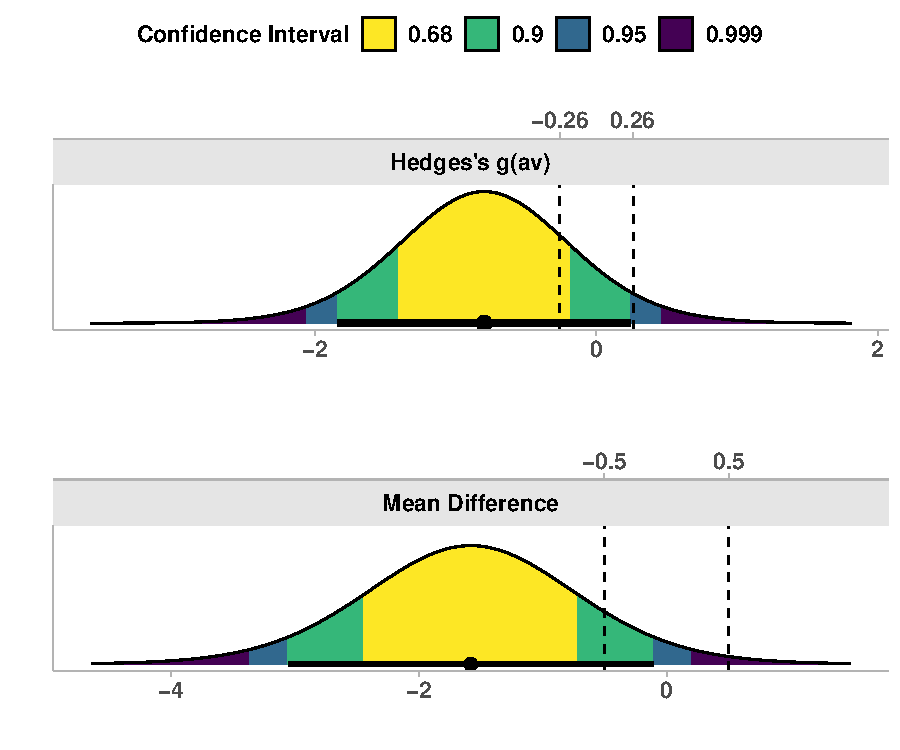
\includegraphics{Avocado_Update_files/figure-latex/cdplot-1.pdf}
\caption{Example of consonance density plot.}
\end{figure}

\newpage

The shading pattern can be modified with the \texttt{ci\_shades}.

\begin{Shaded}
\begin{Highlighting}[]
\FunctionTok{plot}\NormalTok{(res1, }\AttributeTok{type =} \StringTok{"cd"}\NormalTok{,}
     \AttributeTok{ci\_shades =} \FunctionTok{c}\NormalTok{(.}\DecValTok{9}\NormalTok{,.}\DecValTok{95}\NormalTok{))}
\end{Highlighting}
\end{Shaded}

\begin{figure}
\centering
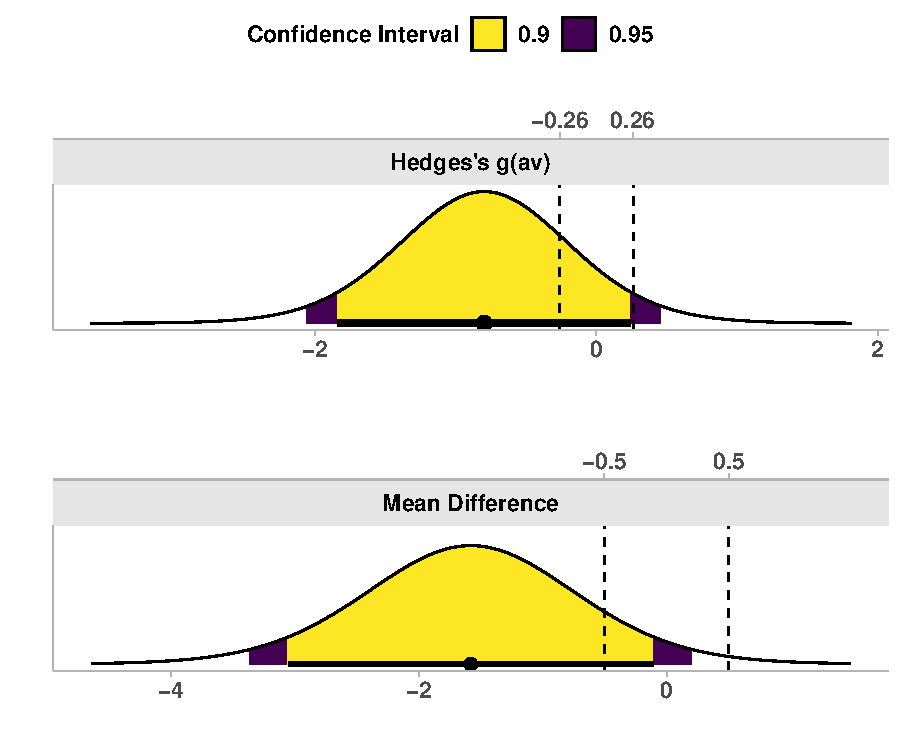
\includegraphics{Avocado_Update_files/figure-latex/shadeplot-1.pdf}
\caption{Demonstrating the shading in plot method.}
\end{figure}

\newpage

Consonance plots, where all confidence intervals can be simultaneous
plotted, can also be produced. The advantage here is multiple confidence
interval lines can plotted at once.

\begin{Shaded}
\begin{Highlighting}[]
\FunctionTok{plot}\NormalTok{(res1, }\AttributeTok{type =} \StringTok{"c"}\NormalTok{,}
     \AttributeTok{ci\_lines =}  \FunctionTok{c}\NormalTok{(.}\DecValTok{9}\NormalTok{,.}\DecValTok{95}\NormalTok{))}
\end{Highlighting}
\end{Shaded}

\begin{figure}
\centering
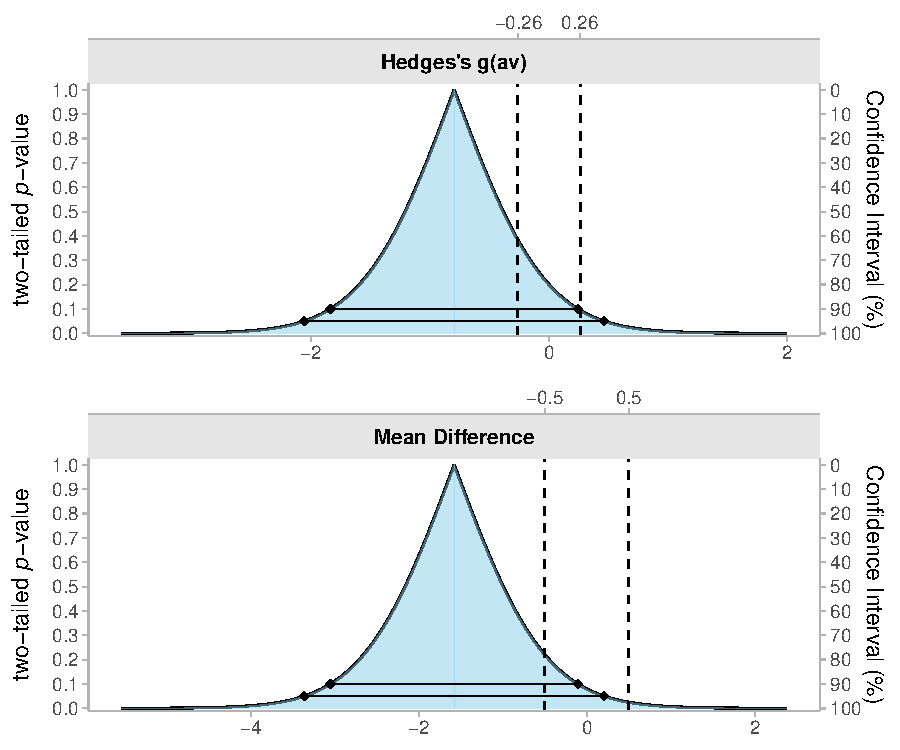
\includegraphics{Avocado_Update_files/figure-latex/conplot-1.pdf}
\caption{Example of consonance plot.}
\end{figure}

\newpage

\hypertarget{paired-samples}{%
\subsubsection{Paired Samples}\label{paired-samples}}

To perform a paired samples TOST, the process does not change much. We
could process the test the same way by providing a formula. All we would
need to then is change \texttt{paired} to TRUE.

\begin{Shaded}
\begin{Highlighting}[]
\NormalTok{res2 }\OtherTok{=} \FunctionTok{t\_TOST}\NormalTok{(}\AttributeTok{formula =}\NormalTok{ extra }\SpecialCharTok{\textasciitilde{}}\NormalTok{ group,}
              \AttributeTok{data =}\NormalTok{ sleep,}
              \AttributeTok{paired =} \ConstantTok{TRUE}\NormalTok{,}
              \AttributeTok{eqb =}\NormalTok{ .}\DecValTok{5}\NormalTok{)}
\NormalTok{res2}
\end{Highlighting}
\end{Shaded}

\begin{verbatim}
## 
## Paired t-test
## 
## The equivalence test was non-significant, t(9) = -2.777, p = 9.89e-01
## The null hypothesis test was significant, t(9) = -4.062, p = 2.83e-03
## NHST: reject null significance hypothesis that the effect is equal to zero 
## TOST: don't reject null equivalence hypothesis
## 
## TOST Results 
##                 t df p.value
## t-test     -4.062  9   0.003
## TOST Lower -2.777  9   0.989
## TOST Upper -5.348  9 < 0.001
## 
## Effect Sizes 
##               Estimate    SE               C.I. Conf. Level
## Raw             -1.580 0.389   [-2.293, -0.867]         0.9
## Hedges's g(z)   -1.174 0.411 [-1.8046, -0.4977]         0.9
## Note: SMD confidence intervals are an approximation. See vignette("SMD_calcs").
\end{verbatim}

\newpage

However, we may have two vectors of data that are paired. So instead we
may want to just provide those separately rather than using a data set
and setting the formula. This can be demonstrated with the ``bugs''
data.

\begin{Shaded}
\begin{Highlighting}[]
\NormalTok{res3 }\OtherTok{=} \FunctionTok{t\_TOST}\NormalTok{(}\AttributeTok{x =}\NormalTok{ bugs}\SpecialCharTok{$}\NormalTok{LDHF,}
              \AttributeTok{y =}\NormalTok{ bugs}\SpecialCharTok{$}\NormalTok{LDLF,}
              \AttributeTok{paired =} \ConstantTok{TRUE}\NormalTok{,}
              \AttributeTok{eqb =} \DecValTok{1}\NormalTok{)}
\NormalTok{res3}
\end{Highlighting}
\end{Shaded}

\begin{verbatim}
## 
## Paired t-test
## 
## The equivalence test was non-significant, t(90) = 2.655, p = 9.95e-01
## The null hypothesis test was significant, t(90) = 6.649, p = 2.22e-09
## NHST: reject null significance hypothesis that the effect is equal to zero 
## TOST: don't reject null equivalence hypothesis
## 
## TOST Results 
##                 t df p.value
## t-test      6.649 90 < 0.001
## TOST Lower 10.642 90 < 0.001
## TOST Upper  2.655 90   0.995
## 
## Effect Sizes 
##               Estimate     SE             C.I. Conf. Level
## Raw             1.6648 0.2504  [1.2487, 2.081]         0.9
## Hedges's g(z)   0.6911 0.1167 [0.4987, 0.8802]         0.9
## Note: SMD confidence intervals are an approximation. See vignette("SMD_calcs").
\end{verbatim}

\newpage

We may want to perform a Minimal Effect Test with the
\texttt{hypothesis} argument set to ``MET''.

\begin{Shaded}
\begin{Highlighting}[]
\NormalTok{res3a }\OtherTok{=} \FunctionTok{t\_TOST}\NormalTok{(}\AttributeTok{x =}\NormalTok{ bugs}\SpecialCharTok{$}\NormalTok{LDHF,}
               \AttributeTok{y =}\NormalTok{ bugs}\SpecialCharTok{$}\NormalTok{LDLF,}
               \AttributeTok{paired =} \ConstantTok{TRUE}\NormalTok{,}
               \AttributeTok{hypothesis =} \StringTok{"MET"}\NormalTok{,}
               \AttributeTok{eqb =} \DecValTok{1}\NormalTok{)}
\NormalTok{res3a}
\end{Highlighting}
\end{Shaded}

\begin{verbatim}
## 
## Paired t-test
## 
## The minimal effect test was significant, t(90) = 10.642, p = 4.69e-03
## The null hypothesis test was significant, t(90) = 6.649, p = 2.22e-09
## NHST: reject null significance hypothesis that the effect is equal to zero 
## TOST: reject null MET hypothesis
## 
## TOST Results 
##                 t df p.value
## t-test      6.649 90 < 0.001
## TOST Lower 10.642 90       1
## TOST Upper  2.655 90   0.005
## 
## Effect Sizes 
##               Estimate     SE             C.I. Conf. Level
## Raw             1.6648 0.2504  [1.2487, 2.081]         0.9
## Hedges's g(z)   0.6911 0.1167 [0.4987, 0.8802]         0.9
## Note: SMD confidence intervals are an approximation. See vignette("SMD_calcs").
\end{verbatim}

\newpage

\hypertarget{one-sample-t-test}{%
\subsubsection{One Sample t-test}\label{one-sample-t-test}}

In other cases we may have a one-sample test. If that is the case, only
\texttt{x} argument for the data is needed. As an example, we may
hypothesis that the mean of LDHF is not more than 1.5 points greater or
less than 7.

\begin{Shaded}
\begin{Highlighting}[]
\NormalTok{res4 }\OtherTok{=} \FunctionTok{t\_TOST}\NormalTok{(}\AttributeTok{x =}\NormalTok{ bugs}\SpecialCharTok{$}\NormalTok{LDHF,}
              \AttributeTok{hypothesis =} \StringTok{"EQU"}\NormalTok{,}
              \AttributeTok{eqb =} \FunctionTok{c}\NormalTok{(}\FloatTok{5.5}\NormalTok{,}\FloatTok{8.5}\NormalTok{))}
\NormalTok{res4}
\end{Highlighting}
\end{Shaded}

\begin{verbatim}
## 
## One Sample t-test
## 
## The equivalence test was significant, t(90) = -4.244, p = 2.66e-05
## The null hypothesis test was significant, t(90) = 27.942, p = 3.91e-46
## NHST: reject null significance hypothesis that the effect is equal to zero 
## TOST: reject null equivalence hypothesis
## 
## TOST Results 
##                 t df p.value
## t-test     27.942 90 < 0.001
## TOST Lower  7.116 90 < 0.001
## TOST Upper -4.244 90 < 0.001
## 
## Effect Sizes 
##            Estimate     SE             C.I. Conf. Level
## Raw           7.379 0.2641  [6.9402, 7.818]         0.9
## Hedges's g    2.905 0.2395 [2.5058, 3.2949]         0.9
## Note: SMD confidence intervals are an approximation. See vignette("SMD_calcs").
\end{verbatim}

\newpage

\hypertarget{using-summary-statistics}{%
\subsubsection{Using Summary
Statistics}\label{using-summary-statistics}}

In some cases you may only have access to the summary statistics.
Therefore, I created a function, \texttt{tsum\_TOST}, to perform the
same tests just based on the summary statistics. This involves providing
the function with a number of different arguments.

\begin{itemize}
\tightlist
\item
  \texttt{n1\ \&\ n2} the sample sizes (only n1 needs to be provided for
  one sample case)
\item
  \texttt{m1\ \&\ m2} the sample means
\item
  \texttt{sd1\ \&\ sd2} the sample standard deviation
\item
  \texttt{r12} the correlation between each if paired is set to TRUE
\end{itemize}

The results from above can be replicated with the \texttt{tsum\_TOST}:

\begin{Shaded}
\begin{Highlighting}[]
\NormalTok{res\_tsum }\OtherTok{=} \FunctionTok{tsum\_TOST}\NormalTok{(}
  \AttributeTok{m1 =} \FunctionTok{mean}\NormalTok{(bugs}\SpecialCharTok{$}\NormalTok{LDHF, }\AttributeTok{na.rm=}\ConstantTok{TRUE}\NormalTok{), }\AttributeTok{sd1 =} \FunctionTok{sd}\NormalTok{(bugs}\SpecialCharTok{$}\NormalTok{LDHF, }\AttributeTok{na.rm=}\ConstantTok{TRUE}\NormalTok{),}
  \AttributeTok{n1 =} \FunctionTok{length}\NormalTok{(}\FunctionTok{na.omit}\NormalTok{(bugs}\SpecialCharTok{$}\NormalTok{LDHF)),}
  \AttributeTok{hypothesis =} \StringTok{"EQU"}\NormalTok{, }\AttributeTok{smd\_ci =} \StringTok{"t"}\NormalTok{, }\AttributeTok{eqb =} \FunctionTok{c}\NormalTok{(}\FloatTok{5.5}\NormalTok{, }\FloatTok{8.5}\NormalTok{)}
\NormalTok{)}

\NormalTok{res\_tsum}
\end{Highlighting}
\end{Shaded}

\begin{verbatim}
## 
## One-sample t-Test
## 
## The equivalence test was significant, t(90) = -4.244, p = 2.66e-05
## The null hypothesis test was significant, t(90) = 27.942, p = 3.91e-46
## NHST: reject null significance hypothesis that the effect is equal to zero 
## TOST: reject null equivalence hypothesis
## 
## TOST Results 
##                 t df p.value
## t-test     27.942 90 < 0.001
## TOST Lower  7.116 90 < 0.001
## TOST Upper -4.244 90 < 0.001
## 
## Effect Sizes 
##            Estimate     SE             C.I. Conf. Level
## Raw           7.379 0.2641  [6.9402, 7.818]         0.9
## Hedges's g    2.905 0.2395 [2.4289, 3.3804]         0.9
## Note: SMD confidence intervals are an approximation. See vignette("SMD_calcs").
\end{verbatim}

\newpage

\hypertarget{robust-methods-for-equivalence-testing}{%
\section{Robust Methods for Equivalence
Testing}\label{robust-methods-for-equivalence-testing}}

In some cases, the use of t-test may be less than ideal. Any serious
violation to the assumptions of a t-test (e.g., normality or
homoscedasticity) could greatly inflate the type 1 error rate of TOST.
Therefore, it may be useful to explore alternatives to the t-test for
TOST.

The TOSTER package currently provides 4 robust alternatives to the
t-test for TOST. First, there is the \texttt{wilcox\_TOST} function
which uses the Wilcoxon-Mann-Whitney (WMW) type tests (i.e.,
\texttt{wilcox.test}) to perform TOST as a test of symmetry. Second,
there is the \texttt{log\_TOST} function which performs log-transformed
t-tests, which is a parametric approach commonly used in pharmaceutical
bioequivalence studies on ratio data \citep{he2022}. Third, there is the
\texttt{boot\_t\_TOST} function which uses the bootstrap method outlined
by \citet{efron93}. Fourth, there is the \texttt{boot\_log\_TOST}
function which uses the same bootstrap method outlined by
\citet{efron93} but on the log-transformed data, which is more robust
than parametric log t-test \citep{he2022}

In the following sections, I will briefly outline the available robust
TOST functions within the TOSTER package.

\hypertarget{tests-of-symmetry-rank-based-tests}{%
\subsection{Tests of Symmetry (rank based
tests)}\label{tests-of-symmetry-rank-based-tests}}

The WMW group of tests (e.g., Mann-Whitney U-test) provide a
non-parametric test of differences between groups, or within samples,
based on \emph{ranks}. This provides a test of location shift, which is
a fancy way of saying differences in the center of the distribution
(i.e., in parametric tests the location is mean). Within the TOST
framework, there are two separate tests of directional location shift to
determine if the location shift is within (equivalence) or outside
(minimal effect) the equivalence bounds. Many researchers mistakenly
think these are tests of medians, but this is not the case (See
\citet{median_test} for details).\footnote{Care should be taken when
  considering paired samples; a test on the rank transformed data
  \citep{kornbrot1990rank} or another robust test may be more prudent.}.
Using a WMW-based TOST is useful for testing whether the differences
between groups/conditions is symmetric around the equivalence bounds.
For equivalence testing, the TOST would be testing whether there is
asymmetry towards no effect with a null hypothesis of symmetry at the
equivalence bound.

In the TOSTER package, we accomplish this ``test of symmetry'' with the
\texttt{wilcox\_TOST} function. This function operates in an extremely
similar implementation to the \texttt{t\_TOST} function. The exact
calculations utilized in this function can be explored via the
documentation of the \texttt{wilcox.test} function. A standardized mean
difference (SMD) is \emph{not} calculated in this function since this
would be an inappropriate measure of effect size alongside the
non-parametric test statistics. Instead, a standardized effect size
(SES) is calculated for \emph{all} types of comparisons (e.g., two
sample, one sample, and paired samples). The function can produce a
rank-biserial correlation (\citet{Kerby_2014}), a WMW Odds
\citep{wmwodds}, or a ``common language effect size''
(\citet{Kerby_2014}) (Also known as the non-parametric probability of
superiority, or concordance probability).\footnote{There is no plotting
  capability at this time for the output of this function.}

As an example, we can use the sleep data to make a non-parametric
comparison of equivalence.

\begin{Shaded}
\begin{Highlighting}[]
\FunctionTok{data}\NormalTok{(}\StringTok{\textquotesingle{}sleep\textquotesingle{}}\NormalTok{)}
\FunctionTok{library}\NormalTok{(TOSTER)}

\NormalTok{test1 }\OtherTok{=} \FunctionTok{wilcox\_TOST}\NormalTok{(}\AttributeTok{formula =}\NormalTok{ extra }\SpecialCharTok{\textasciitilde{}}\NormalTok{ group,}
                      \AttributeTok{data =}\NormalTok{ sleep,}
                      \AttributeTok{paired =} \ConstantTok{FALSE}\NormalTok{,}
                      \AttributeTok{eqb =}\NormalTok{ .}\DecValTok{5}\NormalTok{)}


\FunctionTok{print}\NormalTok{(test1)}
\end{Highlighting}
\end{Shaded}

\begin{verbatim}
## 
## Wilcoxon rank sum test with continuity correction
## 
## The equivalence test was non-significant W = 20.000, p = 8.94e-01
## The null hypothesis test was non-significant W = 25.500, p = 6.93e-02
## NHST: don't reject null significance hypothesis that the effect is equal to zero 
## TOST: don't reject null equivalence hypothesis
## 
## TOST Results 
##            Test Statistic p.value
## NHST                 25.5   0.069
## TOST Lower           34.0   0.894
## TOST Upper           20.0   0.013
## 
## Effect Sizes 
##                           Estimate               C.I. Conf. Level
## Median of Differences       -1.346       [-3.4, -0.1]         0.9
## Rank-Biserial Correlation   -0.490 [-0.7493, -0.1005]         0.9
\end{verbatim}

\hypertarget{bootstrap-tost}{%
\subsection{Bootstrap TOST}\label{bootstrap-tost}}

The bootstrap refers to resampling with replacement and can be used
statistical estimation and inference. Bootsrapping techniques are very
useful because they are considered somewhat robust to the violations of
assumptions for a simple t-test. Therefore we added a bootstrap option,
\texttt{boot\_t\_TOST} to the package to provide another robust
alternative to the \texttt{t\_TOST} function.

In this function we provide a percentile bootstrap solution outlined by
\citet{efron93} (see chapter 16, page 220). The bootstrapped p-values
are derived from the ``studentized'' version of a test of mean
differences \citep{efron93}. Overall, the results should be similar to
the results of \texttt{t\_TOST}. \textbf{However}, for paired samples,
the Cohen's d(rm) effect size \emph{cannot} be calculated by this
function.

\hypertarget{two-sample-algorithm}{%
\subsubsection{Two Sample Algorithm}\label{two-sample-algorithm}}

\begin{enumerate}
\def\labelenumi{\arabic{enumi}.}
\item
  Form B bootstrap data sets from x* and y* wherein x* is sampled with
  replacement from \(\tilde x_1,\tilde x_2, ... \tilde x_n\) and y* is
  sampled with replacement from
  \(\tilde y_1,\tilde y_2, ... \tilde y_n\)
\item
  t is then evaluated on each sample, but the mean of each sample (y or
  x) and the overall average (z) are subtracted from each
\end{enumerate}

\[
t(z^{*b}) = \frac {(\bar x^*-\bar x - \bar z) - (\bar y^*-\bar y - \bar z)}{\sqrt {sd_y^*/n_y + sd_x^*/n_x}}
\]

\begin{enumerate}
\def\labelenumi{\arabic{enumi}.}
\setcounter{enumi}{2}
\tightlist
\item
  An approximate p-value can then be calculated as the number of
  bootstrapped results greater than the observed t-statistic from the
  sample.
\end{enumerate}

\[
p_{boot} = \frac {\#t(z^{*b}) \ge t_{sample}}{B}
\]

The same process is completed for the one sample case but with the one
sample solution for the equation outlined by \(t(z^{*b})\). The paired
sample case in this bootstrap procedure is equivalent to the one sample
solution because the test is based on the difference scores.

\hypertarget{example-of-bootsrapping}{%
\subsubsection{Example of Bootsrapping}\label{example-of-bootsrapping}}

Again, we can use the sleep data to see the bootstrapped results. If you
plot the bootstrap samples, it will show how the resampling via
bootstrapping indicates the instability of Hedges' d(z).

\begin{Shaded}
\begin{Highlighting}[]
\FunctionTok{data}\NormalTok{(}\StringTok{\textquotesingle{}sleep\textquotesingle{}}\NormalTok{)}

\NormalTok{test1 }\OtherTok{=} \FunctionTok{boot\_t\_TOST}\NormalTok{(}\AttributeTok{formula =}\NormalTok{ extra }\SpecialCharTok{\textasciitilde{}}\NormalTok{ group,}
                    \AttributeTok{data =}\NormalTok{ sleep,}
                    \AttributeTok{paired =} \ConstantTok{TRUE}\NormalTok{,}
                    \AttributeTok{eqb =}\NormalTok{ .}\DecValTok{5}\NormalTok{,}
                    \AttributeTok{R =} \DecValTok{999}\NormalTok{)}


\FunctionTok{print}\NormalTok{(test1)}
\end{Highlighting}
\end{Shaded}

\begin{verbatim}
## 
## Bootstrapped Paired t-test
## 
## The equivalence test was non-significant, t(9) = -2.777, p = 1e+00
## The null hypothesis test was significant, t(9) = -4.062, p = 0e+00
## NHST: reject null significance hypothesis that the effect is equal to zero 
## TOST: don't reject null equivalence hypothesis
## 
## TOST Results 
##                 t df p.value
## t-test     -4.062  9 < 0.001
## TOST Lower -2.777  9       1
## TOST Upper -5.348  9 < 0.001
## 
## Effect Sizes 
##               Estimate     SE               C.I. Conf. Level
## Raw             -1.580 0.3816     [-2.28, -1.01]         0.9
## Hedges's g(z)   -1.174 0.6494 [-2.7938, -0.9264]         0.9
## Note: percentile bootstrap method utilized.
\end{verbatim}

\newpage

\hypertarget{log-tost}{%
\subsection{Log TOST}\label{log-tost}}

The logarithmic transformation is often utilized to ``normalize'' the
data or stabilize the variance.

\begin{itemize}
\item
  Basic advantages
\item
  How it translates to a ratio
\item
  FDA requirements
\item
  Default equivalence bounds
\end{itemize}

\hypertarget{example-of-log-tost}{%
\subsection{Example of Log TOST}\label{example-of-log-tost}}

\hypertarget{bootstrap-log-tost}{%
\subsection{Bootstrap Log TOST}\label{bootstrap-log-tost}}

The bootstrap version of \texttt{log\_TOST}, \texttt{boot\_log\_TOST},
using the same bootstrapping method detailed above, but it uses the
log-transformed values

\hypertarget{equivalence-testing-with-anovas}{%
\section{Equivalence Testing with
ANOVAs}\label{equivalence-testing-with-anovas}}

For better or worse, many researchers utilize ANOVA as an omnibus test
for the absence/presence of effects. This is very useful when
implementing factorial designs where multiple experimental factors are
tested and/or manipulated. As \citet{Campbell_2021} suggest, the lack of
a significant result at the ANOVA-level does not necessarily indicate
that a factor or interaction of factors have no effect. However,
\citet{Campbell_2021} only suggest an equivalence test for one-way
ANOVAs and therefore exclude multi-factor ANOVAs. Therefore, I have
extended the work of \citet{Campbell_2021} to include functions that
allow for equivalence testing the partial \(\eta^2\) (eta-squared)
effect size from ANOVAs.

\hypertarget{f-test-calculations}{%
\subsection{F-test Calculations}\label{f-test-calculations}}

Statistical equivalence testing (or ``omnibus non-inferiority testing''
by \citet{Campbell_2021}) for \emph{F}-tests are special use case of the
cumulative distribution function of the non-central \emph{F}
distribution. As \citet{Campbell_2021} states, these type of questions
answer the question: ``Can we reject the hypothesis that the total
proportion of variance in outcome Y attributable to X is greater than or
equal to the equivalence bound \(\Delta\)?''

\hypertarget{hypothesis-tests}{%
\subsubsection{Hypothesis Tests}\label{hypothesis-tests}}

\[
H_0 =  1 > \eta^2_p \geq \Delta
\]

\[
H_1 =  0 \geq \eta^2_p < \Delta
\]

In TOSTER, I have gone a tad farther than \citet{Campbell_2021}, and
calculate a generalization of the non-centrality parameter that allows
the equivalence test for \emph{F}-tests to be applied to variety of
designs.

\citet{Campbell_2021} calculate the \emph{p}-value as:

\[
p = p_f(F; J-1, N-J, \frac{N \cdot \Delta}{1-\Delta})
\]

The non-centrality parameter (ncp = \(\lambda\)) can be calculated with
the equivalence bound and the degrees of freedom:

\[
\lambda_{eq} = \frac{\Delta}{1-\Delta} \cdot(df_1 + df_2 +1)
\]

The \emph{p}-value for the equivalence test (\(p_{eq}\)) could then be
calculated from traditional ANOVA results and the distribution function:

\[
p_{eq} = p_f(F; df_1, df_2, \lambda_{eq})
\]

\hypertarget{example-of-equivalence-anova-test}{%
\subsection{Example of Equivalence ANOVA
Test}\label{example-of-equivalence-anova-test}}

Using the \texttt{InsectSprays} data set in R and the base R
\texttt{aov} function we can demonstrate how this omnibus equivalence
testing can be applied with TOSTER.

From the initial analysis we an see a clear ``significant'' effect (the
p-value listed is zero but it just very small) of the factor spray.
However, we \emph{may} be interested in testing if the effect is
practically equivalent. I will arbitrarily set the equivalence bound to
a partial eta-squared of 0.35 (\(H_0: \eta^2_p > 0.35\))

\begin{Shaded}
\begin{Highlighting}[]
\FunctionTok{library}\NormalTok{(TOSTER)}
\CommentTok{\# Get Data}
\FunctionTok{data}\NormalTok{(}\StringTok{"InsectSprays"}\NormalTok{)}
\CommentTok{\# Build ANOVA}
\NormalTok{aovtest }\OtherTok{=} \FunctionTok{aov}\NormalTok{(count }\SpecialCharTok{\textasciitilde{}}\NormalTok{ spray,}
              \AttributeTok{data =}\NormalTok{ InsectSprays)}

\CommentTok{\# Display overall results}
\NormalTok{knitr}\SpecialCharTok{::}\FunctionTok{kable}\NormalTok{(broom}\SpecialCharTok{::}\FunctionTok{tidy}\NormalTok{(aovtest),}
            \AttributeTok{caption =} \StringTok{"Traditional ANOVA Test"}\NormalTok{)}
\end{Highlighting}
\end{Shaded}

\begin{longtable}[]{@{}lrrrrr@{}}
\caption{Traditional ANOVA Test}\tabularnewline
\toprule()
term & df & sumsq & meansq & statistic & p.value \\
\midrule()
\endfirsthead
\toprule()
term & df & sumsq & meansq & statistic & p.value \\
\midrule()
\endhead
spray & 5 & 2668.833 & 533.76667 & 34.70228 & 0 \\
Residuals & 66 & 1015.167 & 15.38131 & NA & NA \\
\bottomrule()
\end{longtable}

We can then use the information in the table above to perform an
equivalence test using the \texttt{equ\_ftest} function. This function
returns an object of the S3 class \texttt{htest} and the output will
look very familiar to the the t-test. The main difference is the
estimates, and confidence interval, are for partial \(\eta^2_p\).

\begin{Shaded}
\begin{Highlighting}[]
\FunctionTok{equ\_ftest}\NormalTok{(}\AttributeTok{Fstat =} \FloatTok{34.70228}\NormalTok{,}
          \AttributeTok{df1 =} \DecValTok{5}\NormalTok{,}
          \AttributeTok{df2 =} \DecValTok{66}\NormalTok{,}
          \AttributeTok{eqb =} \FloatTok{0.35}\NormalTok{)}
\end{Highlighting}
\end{Shaded}

\begin{verbatim}
## 
##  Equivalence Test from F-test
## 
## data:  Summary Statistics
## F = 34.702, df1 = 5, df2 = 66, p-value = 1
## 95 percent confidence interval:
##  0.5806263 0.7804439
## sample estimates:
## [1] 0.724439
\end{verbatim}

Based on the results above we would conclude there is a significant
effect of ``spray'' and the differences due to spray are \emph{not}
statistically equivalent. In essence, we reject the traditional null
hypothesis of ``no effect'' but accept the null hypothesis of the
equivalence test.

The \texttt{equ\_ftest} is very useful because all you need is very
basic summary statistics. However, if you are doing all your analyses in
R then you can use the \texttt{equ\_anova} function. This function
accepts objects produced from \texttt{stats::aov}, \texttt{car::Anova}
and \texttt{afex::aov\_car} (or any ANOVA from derived from
\texttt{afex}).

\begin{Shaded}
\begin{Highlighting}[]
\FunctionTok{equ\_anova}\NormalTok{(aovtest,}
          \AttributeTok{eqb =} \FloatTok{0.35}\NormalTok{)}
\end{Highlighting}
\end{Shaded}

\begin{verbatim}
##        effect df1 df2  F.value       p.null      pes eqbound     p.equ
## 1 spray         5  66 34.70228 3.182584e-17 0.724439    0.35 0.9999965
\end{verbatim}

\hypertarget{equivalence-between-replication-studies}{%
\section{Equivalence Between Replication
Studies}\label{equivalence-between-replication-studies}}

During the development of the TOSTER update, I was helping advise a team
of researchers on a massive replication project for sport and exercise
science \citep{repSES}. How to determine whether a direct\footnote{Defined
  as being a as-close-as possible replication to the original study. In
  contrast to ``conceptual'' replications.} replication was equivalent
to the original study was common, and contentious, topic of conversation
among the team. Inspired by these discussions, I created 2 functions
that would utilize the basic principles of SMDs\footnote{The textbook by
  \citet{borenstein} and the some of the works of Wolfgang Vietchbauer
  were a large source of information for developing these fucntions.} to
test for differences between two studies.

Overall, the concept is simple: if we have an estimates of SMDs from two
studies we can use large-sample approximation to compute the sampling
variances to estimate the degree to which the two studies differ from
one another.

\hypertarget{conclusions}{%
\section{Conclusions}\label{conclusions}}

\begin{itemize}
\tightlist
\item
  This can be useful.
\item
  This package is not exhaustive but is good for simple analyses and
  teaching
\end{itemize}

\newpage

\hypertarget{additional-information}{%
\section{Additional Information}\label{additional-information}}

\hypertarget{acknowledgements}{%
\subsection*{Acknowledgement(s)}\label{acknowledgements}}
\addcontentsline{toc}{subsection}{Acknowledgement(s)}

I'd would like to thank everyone from the Lakens' laboratory group for
their input and suggestions.

\hypertarget{disclosure-statement}{%
\subsection*{Disclosure statement}\label{disclosure-statement}}
\addcontentsline{toc}{subsection}{Disclosure statement}

The author of this manuscript is the author of the TOSTER package.
Citations of this manuscript will benefit their citation count.

\hypertarget{funding}{%
\subsection*{Funding}\label{funding}}
\addcontentsline{toc}{subsection}{Funding}

No funding was provided for this work.

\hypertarget{notes-on-contributors}{%
\subsection*{Notes on contributor(s)}\label{notes-on-contributors}}
\addcontentsline{toc}{subsection}{Notes on contributor(s)}

Daniel Lakens provided a review of many of the materials that have been
incorporated into the update of TOSTER, and was the original author of
this package.

\hypertarget{nomenclaturenotation}{%
\subsection*{Nomenclature/Notation}\label{nomenclaturenotation}}
\addcontentsline{toc}{subsection}{Nomenclature/Notation}

\begin{itemize}
\tightlist
\item
  ANOVA: Analysis of Variance
\item
  MET: Minimal Effects Test
\item
  ncp: non-centrality parameter
\item
  SMD: Standardized mean difference (e.g., Cohen's d)
\item
  TOST: Two-one sided tests
\item
  WMW: Wilcoxon-Mann-Whitney
\end{itemize}

\hypertarget{notes}{%
\subsection*{Notes}\label{notes}}
\addcontentsline{toc}{subsection}{Notes}

The R package is also (partially) implemented in jamovi as the TOSTER
module.

\newpage

\bibliographystyle{tfcad}
\bibliography{interactcadsample.bib}





\end{document}
